%
% Chapter 4
%

\chapter{Monte Carlo Event Generation}
\label{chap:event_sim}

\section{Introduction}

Accurate simulations for signal and backgrounds are needed for searches for new physics. The primary collision along with the decay processes in an event can be described by perturbative quantum field theory. However, perturbative QCD (pQCD) cannot describe the quantum chromodynamics (QCD) bound states. Therefore phenomenological models are needed to describe hadronization.

Event generators are used for generating simulated particle physics events. Event generators factorize the full process of the event simulation into individual tasks. Monte Carlo (MC) methods are used for the probabilistic branching between these individual problems. MC methods are a class of computational algorithms that rely on repeated random sampling to have the same average behaviour in simulation as in collision data. Event signature of beyond standard model particles an be generated to compare its signature to the one of generated background processes.

General-purpose Monte Carlo (GPMC) generators, like PYTHIA \cite{Sjostrand:2014zea}, provide fully exclusive simulations of high-energy collisions. However, there are also event generators which are specialised on a certain aspect of the event simulation. Perturbative matrix elements for the scattering process are implemented in matrix element generators. Hadronic event generators simulate the initial- and final-state particle showers, hadronization, and soft hadron-hadron physics including composition and substructure of the initial state. An overview of different steps in MC generation for proton-proton collision events can be seen in Figure \ref{fig:simulation}.

\begin{figure}[htbp]
  \centering
  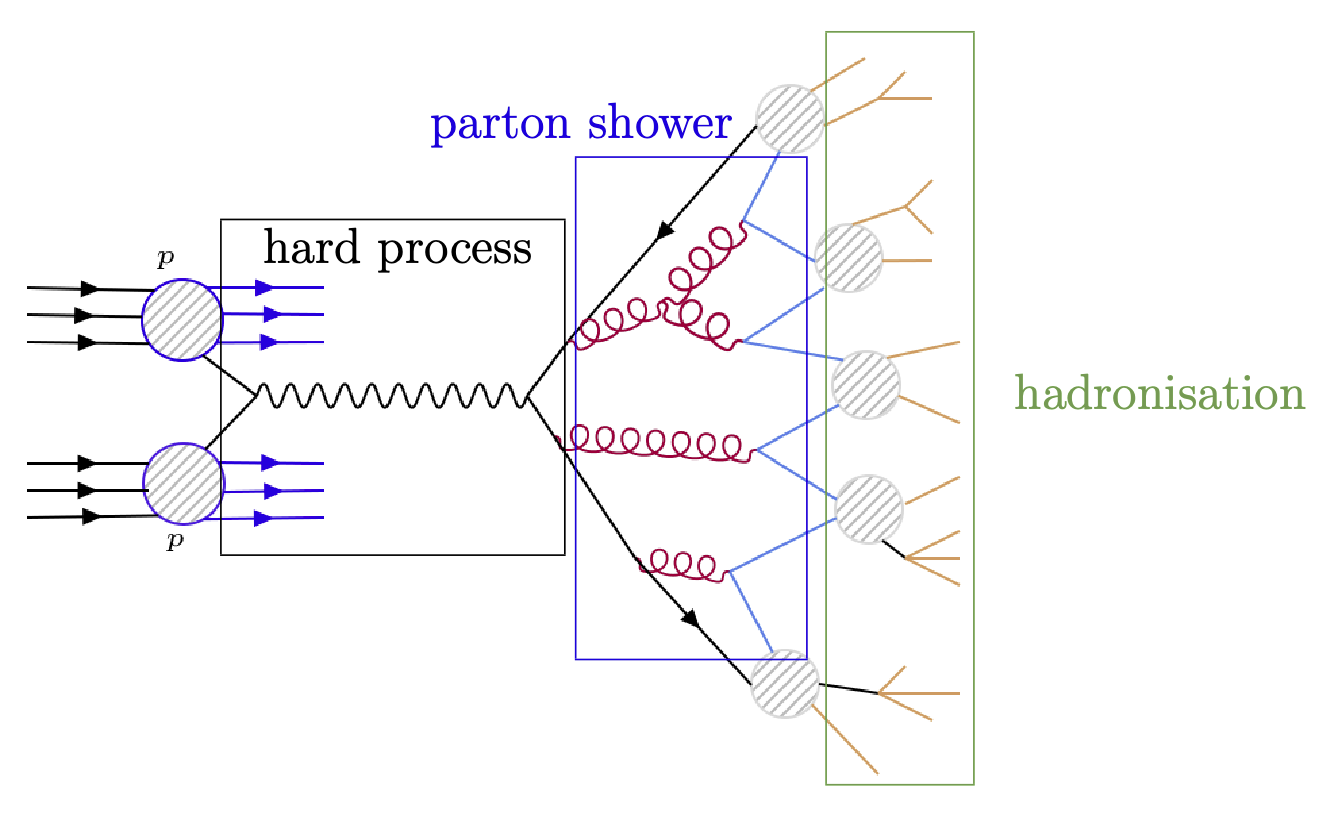
\includegraphics[width=0.8\textwidth]{plots/chapter4/simulation.png}
  \caption{Monte Carlo simulation of an event in proton-proton collisions.}
  \label{fig:simulation}
\end{figure}

In the following sections, first, the simulation of short distance processes is described. In these processes the momentum scales are high enough to use perturbative quantum chromodynamics for the description of the strong interaction between quarks and gluons. Next, quarks fragmention into composite particles called hadrons is described using the hadronization models. This is followed by soft hadron-hadron physics modelling and tuning.

First, the simulation of short distances processes is described, where the momentum scales are high enough to use perturbative quantum chromodynamics for the description of the strong interaction between quarks and gluons. Afterwards, hadronisation models are discussed which become important at lower energy scales, where quarks fragment into composite particles called hadrons. Soft hadron-hadron physics modelling, parameters and tuning are introduced. Lastly, the Monte Carlo generators that are important for the current analysis are presented along with the simulation of the detector response.


\section{Perturbative simulation}

The primary hard interaction process along with the decay of short-lived particles happen at short-distance scales. The QCD and quantum electrodynamics (QED) radiation at time scales much below $\frac{1}{\Lambda}$, where $\Lambda$ is a typical hadronic scale of a few hundred MeV are also happening at short-distance scales. Soft- and collinear-safe inclusive observables, such as total decay widths or inclusive cross sections, can be computed with pQCD theory for momentum scales much larger than this scale. The final-state collinear splittings and soft emissions give rise to large logarithmically divergent corrections which cancel against virtual corrections in the total cross section. Initial state collinear singularities are factorised into parton density functions (PDFs). Therefore the crosssection for the process remains accurate up to higher order corrections if it is interpreted as inclusive crosssection. If this is not the case then the singularities in QCD can lead to a non-convergence of the fixed-order expansion.

Matrix-element generators generate the matrix element of the hard process and large-angle emissions. The parton showers are generated by hadronic event generators using collinear and soft radiation approximations. Parton-level events are transferred from a hard-process generator to a shower generator, containing a list of particles and the used free parameters, using the Les Houches Event File (LHEF) standard \cite{Alwall:2006yp}.

\subsection{Matrix element generators}

Matrix element generators generate the exact matrix elements for the production of the process. They also produce a certain number of additional partons for hard, large-angle emissions. The radiation of extra partons is not included at tree-level accuracy of the hard process. The radiation of an extra parton with tree-level accuracy can be included to provide Next-to-leading order (NLO) corrections along with all NLO virtual corrections. The parton shower algorithms use as input the final-state partons of the hard process and their phase space.

\subsection{Parton shower algorithm}

The parton shower algorithm is used for computing the cross section for a generic hard process. The kinematics of the basic process are first generated, followed by a sequence of independent shower splittings. Sudakov form factors $\Delta_{i}(t, t')$ \cite{Collins:1989bt}, are used for estimating the probability for undergoing a branching before the infrared cut-off for each primary process parton i. The infrared cut-off is defined by the decay width for an unstable particle or the shower hadronization scale. Sudakov form factor is interpreted as the probability for a splitting not to occur between two scales $t < t'$. The parton is either split into two partons or the parton is defined as final parton. Altarelli-Parisi splitting kernels \cite{Altarelli:1977zs} define the probability of the parent parton i, with energy fraction z, to decay into two partons j and k. All generated partons undergo this procedure recursively and the algorithm stops when no final-state parton undergoes further splitting.

At each splitting vertex we can assign the azimuthal angle $\phi$ of the splitting process with respect to the incoming parton momentum, the energy fractions $z$ of the two partons, and an ordering variable for the purpose of ordering the parton splittings. PYTHIA uses the imparted transverse momentum $p_{\perp}$. The cross section for the given final state is calculated by assigning a probability to each splitting vertex. Collinear emission and emissions of soft gluons at arbitrary angles are the two sources of infrared singularities in massless field theories like QCD. PYTHIA uses a $p_{\perp}$-ordered shower evolution for correctly describing both effects. There is also an angular veto to avoid the particle multiplicity growing too rapidly with energy.

A cut-off for collinear radiation is obtained from quark masses larger than $\Lambda$, like c, b, or t quarks. For angles between both produced partons $\theta < \theta_{0} = \frac{m_q}{E}$, where $m_q$ is the quark mass and $E$ is the energy, the divergent behaviour is regulated. Heavy quarks have less collinear activity than light quarks. Therefore, in the hard process a larger fraction of the momentum acquired is carried by them. A matrix-element correction method is used by PYTHIA to include the mass effects. PYTHIA does not take the spin correlations into account when generating the parton showers. The initial-state radiation (ISR) has to be taken into account and it induces a nonvanishing transverse momentum of the particles in the matrix element. ISR is taken into account using backwards evolution algorithms.

Photon emission from light charged particles are also added by shower algorithms to account for electromagnetic corrections. For electrons, soft photon emission is especially important. A cut-off for the electromagnetic shower is used to terminate the algorithm. This cut-off is the electron mass in the case of electrons and for quarks, the photon wavelength has to be smaller than the typical hadronic size of about 1 fm. Additional bremsstrahlung can be produced from hadron and tau decays involving charged particles.

The production and decay of particles are treated as being factorisable. The distribution of the mass along with the distributions of its decay products are relevant. A $\delta$ function at pole mass $m_0$ or a Breit-Wigner distribution with particle width $\Gamma$ can be used for mass distribution. Differential decay matrix elements or the pole mass and a uniform phase-space distribution can be used for describing the decay products. The total invariant mass of the decay products is preserved by most parton-shower models to keep the original resonance shape.

\subsection{Matching}

QCD color confinement restricts quraks and gluons from existing as isolated particles. The hadronisation of a quark or a gluon gives rise to hadrons or their decay products. Jets are collimated bunches of these hadrons. The collinear/soft-radiation of an appropriate (N + 1)-parton final state, generated by a matrix element generator, can give rise to a (N + 1)-jet event. A (N + 1)-jet event can also be obtained from an N-parton final-state with hard, large-angle emission during shower evolution. A matching has to be done if different generators have been used for generating matrix-elements and parton showers or extra partons have been generated by the hard-process generator.

The exact matrix elements for the production of the basic process and up to n partons are generated by the matrix element generator. At large angles they are tree-level accurate and match the results of the shower algorithms at small angle. The relative transverse momentum is above a scale $Q_{cut}$ for each produced parton pair. There are no final states with more partons and no emissions below the scale $Q_{cut}$.

The hadronic event generator generates events with less than these n additional partons and splittings for scales below $Q_{cut}$. Splittings are also generated for initial events with n partons for relative transverse momenta below the scale of smallest pair momentum $Q_{cut}$. For fixed-order perturbation theory to hold, the matching parameter $Q_{cut}$ has to be large enough. However, the $Q_{cut}$ also has to be small enough so that the shower algorithm is accurate for emissions below it. Consistent coupling constant, \as, choices between real and virtual corrections have to be used.

To avoid phase-space double-counting as well as unpopulated phase-space regions matching schemes \cite{Hoche:2006ph} are used. These schemes define which of both paths should be generated for a given event. The choice of the path is optimised to use the best possible approximation to given kinematics. For the production of final state X and n jets, a jet measure is defined and all cross sections are calculated. Hard parton samples are then generated with a probability according to the total cross section and the matrix element. A dynamical, kinematics-dependent probability is used to accept or reject the events. The parton shower is finally invoked and no extra jets are produced with it.


\section{Hadronisation models}

The hadronisation scale $Q_{had}$ is by construction equal to the infrared cut-off where the parton shower ends. Coloured partons are transformed into a set of colourless hadrons by GPMCs. This happens at scales with low momentum transfers and at long distances, where non-perturbative effects become important. QCD inspired models which rely on the colour-flow information between partons are used by GPMCs as starting point for hadronisation. The probability distribution for the hadron energy fraction from coloured partons is given by fragmentation functions.

\subsection{Fragmentation function}

Fragmentation functions are probability distributions for inclusive hadron spectra. They can be calculated using pQCD and a non-perturbative initial condition obtained by fitting hadron spectra and are defined at an arbitrary perturbative scale Q. More information is included in the MC modelling and is exclusive, while the fragmentation function only describes inclusive spectra \cite{Peterson:1982ak}.

\subsection{String model}

String models are based on ``linear confinement''. In quenched lattice QCD, at distances greater than a femtometre the potential of the colour-dipole field between a colour charge and an anticharge appears to grow linearly with charge separation. One such model os the Lund model. Parton showering gives rise to color-connected quark-antiquark pairs. As the string grows, the non-perturbative creations of new quark-antiquark pairs are favoured, which break the string in two new strings. Kinks are used for representing intermediate gluons which can also be involved, building a transverse structure in the one-dimensional object, while innitely soft gluons are absorbed into the string. When a string breaks they are causally disconnected.

In the Lund model, starting with the leading hadrons the string breaks are generated, containing the endpoint quarks, iterating inwards to the centre of the string, alternating between both sides. In each step, a single on-shell hadron can be split off. After the breakup process the quarks can acquire a transverse momentum $p_{\perp}$. $m_{q}$ and $p_{\perp}$ are used for exponentially suppressed production of quarks. Strangeness can be generated in the parton shower through perturbative $g \to s\bar{s}$ splittings. Baryons can be produced by allowing string breaks to a pairs of diquarks. The relative rate of diquark to quark production can be extracted from collision measurements of ratio of proton to pion.

The produced quarks are assigned to hadron multiplets. As the individual rates are not predicted by the model there are many free parameters. The ratio of vector to pseudoscalar production is another parameter. The fraction $z$ of the quark longitudinal-momentum carried by the created hadron is estimated using the Lund symmetric fragmentation function. Heavier flavoured hadrons carry a larger momentum fraction $z$ of the heavy quark \cite{Bjorken:1977md}, therefore their fragmentation functions should be harder than a light hadron.

\subsection{Hadron and tau decays}

Many primary hadrons originating from string breaks are unstable and decay further until a set of particles is obtained which is stable on relevant time scales. The final particle yields and spectra have a significant impacts from the decay modelling. The summary of available experimental measurements are represented in particle summary tables. Charmed hadron decays have been measured at different experiments and all measured branching ratios do not have to sum to unity. However, MC simulations need decay packages with quantified, consistent information, with all branching fractions adding up to unity. Hence, choices have to be made when adapting summary tables and double counting has to be avoided. The differential distribution of the decay products in phase space also needs to be decided. For a selected class of decays matrix elements can be used. It depends on the generator if additional effects, such as B-meson oscillations, or CP-violating effects, are included.


\section{Soft hadron-hadron physics modelling}

Underlying Event (UE) is the additional activity beyond the basic process and its associated ISR and FSR activity. The dominant part is coming from additional colour exchanges between the beam remnants. Multiple parton-parton interactions (MPI) can produce two or more back-to-back jet pairs with each pair having a small transverse momentum. This is in contrast to jets coming from bremsstrahlung which tend to be aligned with their parent parton. Most MPI are soft and they influence the colour flow and the total scattered energy of the event. This increases the the particle multiplicity in the final state and affects the final-state activity. Compared to events with no hard jets, the hard jets appear to sit on top of a higher "pedestal" of underlying activity. This comes from the impact parameter-dependence, since central collisions are more likely to contain at least one hard scattering due to the higher probability of interactions and is called the "jet pedestal" effect. Therefore, the impact-parameter shape is another free parameter.


\section{Parameter Tuning}

The accuracy of the used models is very important for event simulation. The accuracy depends on the inclusiveness of the chosen observables and on the sophistication of the simulation. The models can be improved by improving the theoretical calculations. The precision also depends on the constraints in the free parameters and existing collision data is used to constrain them and is referred to as generator tuning. MC generators are not tuned beyond the constraints in theoretical and experimental precision due to overfitting. Otherwise it would describe fluctuations or noise instead of the underlying relationship. PDFs for the evolution probability for ISR, \as, properties of non-perturbative fragmentation functions, the matching parameter Qcut and the hadronisation scale Qhad are the parameters. Other parameters are the production rates of mesons and baryons, including the ratio of vector to pseudoscalar production, their masses and decay widths. The largest amount of free parameters are from these parameters and the parameters of the decay modelling. If significant changes to decay treatment are made then the hadronisation parameters should be retuned. As discussed for the underlying event activity and the jet-pedestal shape, the impact parameter shape of the beam particles is an important parameter. The final state y the particles and their spectra are influenced by event modelling and the generator tuning. Events generated with different generators or tunes can be different and might not describe the collision data in the entire phase space.


\section{Monte Carlo generators}

GPMC generators like PYTHIA can simulate the full process. However, there are specialized generators which deal with a certain aspect of the event simulation. MadGraph 5 generates the matrix element with leading-order (LO) accuracy \cite{Alwall:2011uj}. MadGraph 5 is a matrix element generator for processes that involve final states with a large number of jets, heavy flavor quarks, leptons and missing energy. Events from new physics models which are renormalisable or from an effective field theory that can be written in form of a Lagrangian can be generated. The Feynman rules from a given input Lagrangian are derived using FeynRules \cite{Christensen:2008py}. The Feynman diagrams are generated and the code is computed which is necessary to evaluate the matrix element at a given phase-space point for a process using the Feynman rules. Valid diagrams are constructed by the diagram generation algorithm which recursively generates all diagrams in parallel reusing already calculated subdiagrams. Wave functions can be reused when they correspond to identical subdiagrams, but contribute to different diagrams. For each fermion line in a diagram, a fermion flow is defined. Fermions are grouped in pairs with each constituting a fermion line. For states which are charged under SU(3)C, the color coefficients in scattering amplitudes are computed. Multiparton amplitudes are important as they correspond to leading order approximation of multi-jet production. The full amplitude is split into gauge invariant subamplitudes. The matrix element that results contains the full spin correlation and Breit-Wigner effects, but are not valid far from the mass peak.

POWHEG is a framework for implementing next-to-leading order (NLO) matrix-element calculations \cite{Alioli:2010xd}. It includes NLO virtual corrections and radiation of an extra parton in the matrix element. POWHEG method has been applied to several hard processes, including single top production, \ttbar production and Higgs production via gluon fusion, vector boson fusion, and Higgs boson fusion production associated with a vector boson (Higgs strahlung). It needs the LO matrix-elements and the finite part of the virtual corrections as input from which it finds all the singular regions. Using the Frixione, Kunszt and Signer (FKS) subtraction scheme \cite{Frixione:1995ms, Frixione:1997np} the real cross section is split into a sum of contributions that are divergent in one singular region. The singular regions are characterised by final-state parton becoming collinear or soft to either an initial-state parton or a final-state parton. The singular regions can be grouped according to their underlying LO-diagram by replacing this parton pair with a single parton of appropriate flavor. Soft and collinear counterterms as well as remnants are built after finding all singular regions. The POWHEG Sudakov form factor are used for generating the radiation. When no radiation is generated, Born-like events are generated. Below a threshold gluon splittings into heavy quark pairs are avoided. The incoming and outgoing partons are assigned color on basis of the underlying LO-process and to the real emitter and the radiated parton. Since the resonance mass must be preserved by the shower, the information on intermediate resonances is made available to the shower program along with the decay products being specied. The flavor structure has one more light parton in its final state and colourless and massive coloured particles remain the same at LO and NLO level. The interference of LO and one-loop amplitude, have the same flavor structure as the LO term.

aMC@NLO implements all aspects of NLO computation and its matching with parton showers \cite{Frederix:2011ss, Alwall:2014hca}. NLO calculations can be achieved by combining the computation of one-loop matrix elements and tree-level matrix elements. Tree-level computations are performed using MadGraph and one-loop amplitudes are evaluated with MadLoop \cite{Hirschi:2011pa}. The undesirable large short-scale effects can be removed by MC counterterms. They also set an upper bound for the hardness of each branching. Matched samples, which differ by their final-state multiplicity, can be merged using the FxFx- merging scheme.

MLM matching scheme is a matching algorithm \cite{Mangano:2001xp, Mangano:2002ea} that matches partons from matrix element calculations to jets reconstructed after shower generation. Parton-level events are required to have a separation greater than a minimum value $R_{jj} > R_{min}$ between them and at least a minimum transverse energy $E^{min}_{T}$ for partons. These events do not any hard-emission veto during shower. Starting with the hardest parton, the jet closest in $(\eta, \phi)$ is selected and both match if the distance is smaller than $R_{min}$. Once a match is found the jet is removed and matching is done with the next parton. If a match is not found then the event is rejected. This is the case for collinear partons or soft partons, which do not lead to an independent jet or are too soft for jet reconstruction.

FxFx merging scheme is an NLO merging procedure \cite{Frederix:2012ps}. There can be NLO accuracy for exclusive events with J light jets by the computation based on matrix elements that have J and (J + 1) partons. NLO mergings are more complicated than LO ones. This is because the matrix elements are considered twice, as Born contribution for processes with J partons, and as real-emission contribution, IR subtraction terms, and the one-loop contributions to a processes with (J - 1) partons. Double counting is avoided by parton-shower dependent MC counterterms and Sudakov reweighting, as Sudakov form factors include virtual corrections and non-emission probabilities. The parton shower dominates at soft scales, while the contributions from the matrix element dominate at hard scales. At intermediate scales a probability function estimates which description is more accurate. There is no emission larger than the matching scale generated by shower. Events are reweighted and a certain amount of events might carry negative weights.

PYTHIA 8 has been developed for multiparticle production in $e^{+}e^{-}$, $pp$ and $ep$ collisions and simulation of jets. PYTHIA can generate the hard subprocess, initial- andnal-state parton showers, hadronisation, decays and the underlying event. A lot of hard processes have been implemented for generating the matrix elements for final-state and phase space calculation. $2 \to 1$ and $2 \to 2$ processes can be optimally generated by PYTHIA. Resonance decays with the resonance masses above the b-quark system are implemented. Their branching fractions and partial width can be dynamically calculated as function of their mass. If the spin information is available for resonance decays it leads to properly correlated angular correlations of the resonance decay products, otherwise the resonance decays isotropically.

A multijet structure is added by the parton shower which does not take into account the spin effects. Showers are ordered by their virtuality $p_{\perp}$. The initial-state showering is done by a backward evolution scheme. The shower is traced backwards in time starting from the incoming parton of the hard interaction to find the parton which initiated the shower. PYTHIA 8 uses Dipole showering. Gluon emission is generated via dipole radiation rather than by splitting partons. FSR are associated with dipoles which are stretched between the "hole" left by an initial-state parton and a final-state parton. The hard scattering subsystem takes the recoil having initial-state radiation unchanged. Lund string model is used for implementing the Hadronization. The process is split into generating the fragmentation and the decays of these hadrons.


\section{Detector simulation}

In detector simulation, the interactions of particles with the detector material and the detector response are simulated. These events can then be reconstructed and analysed. Geant4 \cite{Agostinelli:2002hh} is used for detector simulation. It is a toolkit for simulating passage of particles through matter and for simulating particle interactions with matter across a very wide energy range. The user defines the detector geometry and materials. A large number of components with different shape and materials can be included in the geometrical model. Sensitive elements can be defined which record information in the form of hits. Hits are needed to simulate the detector responses called digitisation. The detector's geometrical structure is divided into logical and physical volumes. Logical volumes contain the information of the material and the sensitive detector behaviour. A mixture of different elements and isotopes can be used for the material. Physical volumes carry information about the spatial positioning or placement of the logical volumes.

Particles can interact with the detector material or can decay while they are transported through the geometry. A model can be implemented by electromagnetic and hadronic processes in Geant4 depending on the energy or particle type. Geant4 can handle ionisation described by energy loss and range tables, bremsstrahlung, pair production of electron-positrons from muons, photo-electric effect, pair conversion, annihilation, synchrotron and transition radiation, scintillation, refraction, reflection, absorption, the Cherenkov effect, and many other processes. Particles with their basic properties, like mass, charge, list of sensitive processes, can be defined. Particles are transported in steps and they are tracked through materials and external electromagnetic fields. Event data is generated during simulation. First, events contain primary vertices and primary particles before processing an event. After processing, hits and digitisations generated by simulation are added. Trajectories of simulated particles can be added optionally for recording of "simulation truth".
